% Chapter Template

\chapter{Ρομποτική Πλατφόρμα} % Main chapter title


\label{Chapter2} % Change X to a consecutive number; for referencing this chapter elsewhere, use \ref{ChapterX}

%----------------------------------------------------------------------------------------
%	SECTION 1
%----------------------------------------------------------------------------------------

\section{Το Ρομποτικό Όχημα Monstertruck}
Το ρομποτικό όχημα Monstertruck αποτελεί μία ρομποτική πλατφόρμα, που αναπτύχθηκε στα πλαίσια της ομάδας P.A.N.D.O.R.A., για συμμετοχή σε διαγωνισμό με θεματολογία την διάσωση θυμάτων σε συνθήκες καταστροφής. Η ρομποτική πλατφόρμα είναι κατάλληλη για εφαρμογές χαρτογράφησης, εξερεύνησης άγνωστων χώρων και αναζήτησης σημείων ενδιαφέροντος, όπως για παράδειγμα, ανθρώπινα θύματα.\\

Για την κατασκευή της ρομποτικής πλατφόρμας, χρησιμποιήθηκε, σαν βάση, το τηλεκατευθυνόμενο όχημα GroundPounder της εταιρείας Redcat Racing. Ανήκει στην κατηγορία φορτηγών οχημάτων Monstertruck, με κλίμακα 1:10 και περιλαμβάνει σκελετό από αλουμίνιο, τετρακίνηση, όπως επίσης, και αναρτήσεις. Επιπλέον, περιλαμβάνει δύο σερβοκινητήρες, για τον ανεξάρτητο έλεγχο στρέψης των μπροστινών και πίσω τροχών, κάτι το οποίο, δίνει μεγαλύτερη ευελιξία, σε σχέση με τα συμβατικά αυτοκίνητα.

\begin{figure}[!h]
	\begin{center}
		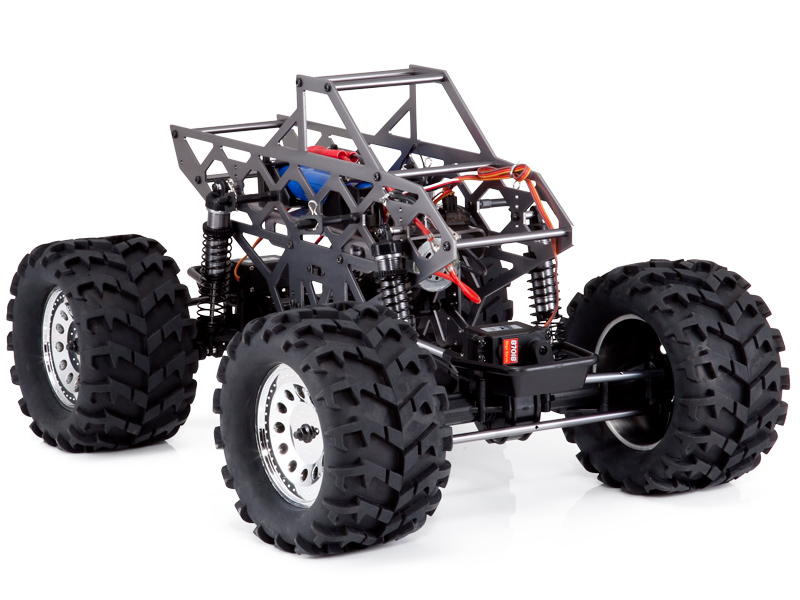
\includegraphics[width=10cm]{Chapters/Chapter2/Figures/groundpounder_chassis.jpg}
		\caption{Το τηλεκατευθυνόμενο όχημα 1:10 GroundPounder}
		\label{fig:groundpounder_chassis}
	\end{center}
\end{figure}


 